\documentclass[10pt,aspectratio=169]{beamer}


  \usetheme{NYU}      % or try Darmstadt, Madrid, Warsaw, ...
  \usecolortheme{default} % or try albatross, beaver, crane, ...
  \usefonttheme{default}  % or try serif, structurebold, ...
  \setbeamertemplate{navigation symbols}{}
  \setbeamertemplate{caption}[numbered]
\usepackage{appendixnumberbeamer}
\usepackage{mymacro}


\newcommand{\ind}{\perp\!\!\!\!\perp} 
\usepackage{hyperref}
\usepackage{minted}
\usepackage[round]{natbib}

\hypersetup{
    colorlinks=blue,
    linkcolor=blue,
    filecolor=blue,      
    urlcolor=blue,
    citecolor=blue,
}

% If you want to print handouts
%\documentclass[handout]{beamer}

% Changing the fonts: this will make the slides more readable and the math look like regular tex math
%\usefonttheme{arial}

% Titles will appear in Small Cap Serif



% -----------------------------------------
% Center the Frame Title
% -----------------------------------------




% -----------------------------------------
% Number the slides
% -----------------------------------------

\setbeamertemplate{footline}[frame number]

% -----------------------------------------
% Get rid of the irritating navigation bar
% -----------------------------------------

\setbeamertemplate{navigation symbols}{}
% -----------------------------------------
% Begin Document
% -----------------------------------------
\title{\Large\textsc{The 4T Will Not Be Televised, It Will Be Livestreamed: Censorship and Narrative Control in Mexico}}
\author[Zago] % Esto es lo que sale en el footer
{\textbf{Eduardo Zago}\inst{1}  \vspace{10pt}}

\institute []% Esto es lo que sale en el footer
{  \inst{1}   PhD Student NYU Politics}

\date{\textsc{}}

\titlegraphic{\hfill\includegraphics[height=1.5cm]{nyu_stacked_color}}


\begin{document}
\maketitle
%  I separate each slide with a line:

% -----------------------------------------

%  I start with the screen black, like using the b key in Powerpoint



% -----------------------------------------
%  Restore normal white background

\beamersetaveragebackground{white}


% -----------------------------------------

%  Example of a slide with animated math:
\section{Motivation}


\begin{frame}{Why Governments Hold Interactions with Media?}
\begin{itemize}
  \setlength\itemsep{1em}

    \item Globally, governments increasingly trying to speak \alert{directly} to audiences and to \alert{manage press access} through controlled formats (press pools, livestreams, social media).
    \item President Trump has had more exchanges with the press than 6 predecessors {\footnotesize\color{gray}\citep{Trump100Days}}. 
    \item Also, Andres Manuel Lopez Obrador (AMLO), ex-president of Mexico held 1,423 2-hour press conferences during his tenure.
    \item \textbf{Broadly, I would like to shed some light on what are the incentives (and costs) of both, the government and the media, to have these recurrent interactions?}

    
\end{itemize}
\end{frame}

%%%%%%%%%%%%%%%%%%%%%%%%%%%%%%%%%%%%%%%

\section{Background}


\begin{frame}{Why Governments Hold Interactions with Media?}
\begin{itemize}
  \setlength\itemsep{1em}


  \item Following his 2018 victory, President L\'opez Obrador (AMLO) created a direct-to-public communication channel: the \textbf{\textit{Mañanera}}.

  \item The \textit{Mañanera} is a daily agenda-setting press conference where access to the microphone depends heavily on \textbf{visibility and physical proximity} (front rows).

  \item Initially, a ``first-come, first-served'' rule generated \textbf{adverse selection of questioners}: front-row access became concentrated among aligned outlets, limiting critical questioning and undermining perceived credibility (or anecdotal evidence seem to suggest \citep{Tombola-Razon})

  \item In April 2022, the administration introduced a \alert{daily seat lottery} for the first three rows to broaden access and restore engagement.
\end{itemize}
\end{frame}

\begin{frame}{Why Standard Classification May Fail}
\small
\begin{itemize}\setlength\itemsep{0.6em}
    \item In this presentation I will focus on a measurement issue relate to this project: measuring dissent with a time-varying and relevant context
    \item A question that looks \textit{neutral} in isolation may be \textbf{oppositional} in context --- and vice versa: a question that sounds \textit{critical} may simply follow the government agenda.
    
    \item Standard classifiers treat each question as an \textbf{isolated document}. But in this setting, classification is inherently \textbf{context-dependent}.
    
    \item This is consistent with work showing that linguistic meaning shifts over time, and stance classification becomes harder when context changes. \citep{mu2024examining, li2023stance, sucu2025exploiting}
    
    \item So the empirical challenge is:
    \[
    \text{Question text} \;+\; \text{day-specific information environment}
    \;\Rightarrow\; \text{alignment/dissent}
    \]
\end{itemize}
\end{frame}

%%%%%%%%%%%%%%%%%%%%%%%%%%%%%%%%%%%%%%%%

\begin{frame}
    \begin{figure}
        \centering
        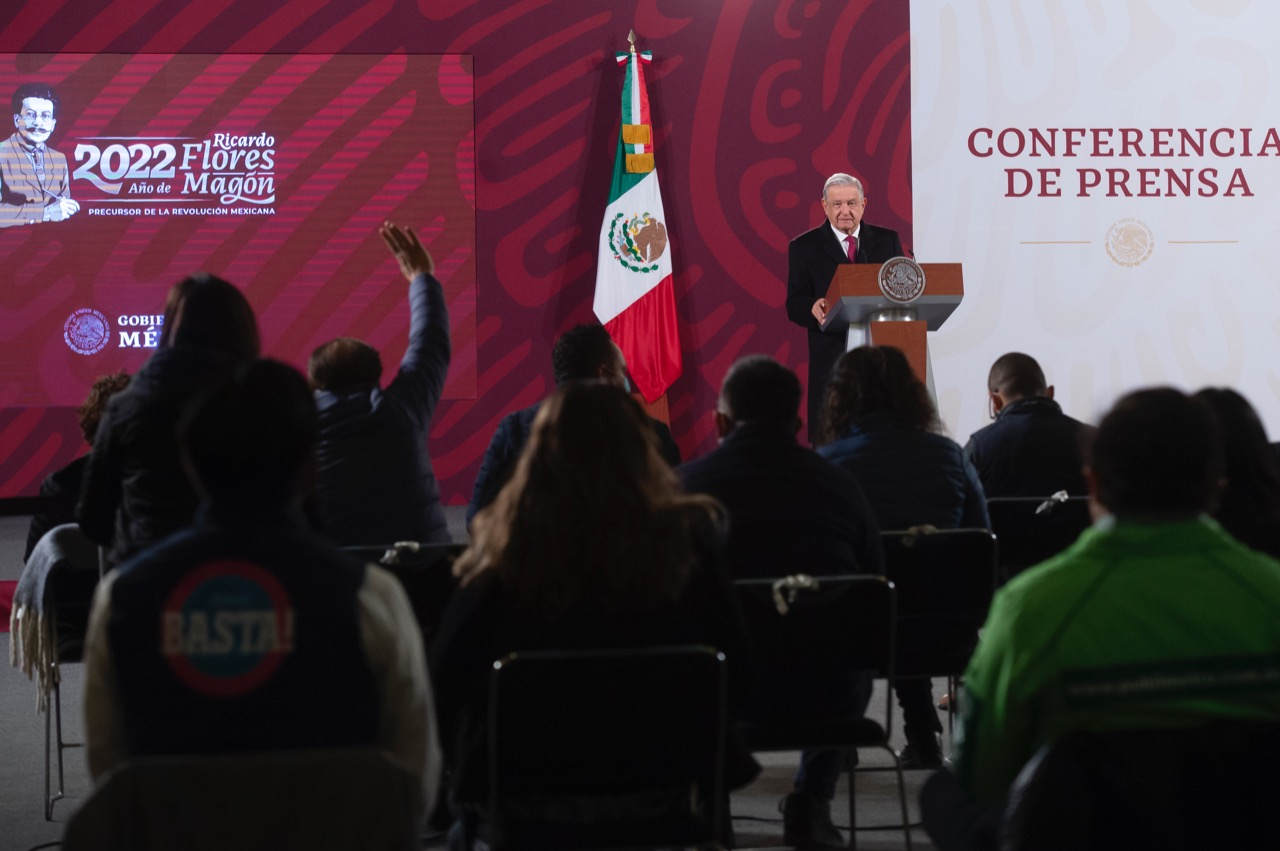
\includegraphics[width=.8\textwidth]{figures/descriptive_stats/mañanera_ex.jpeg}
        \vspace{-0.2cm}
        \caption{\scriptsize Example of a Mañanera}
    \end{figure}
\end{frame}

\section{Why this is important?}

% --- First slide in section: Why this is important? ----------------------------

\begin{frame}
\frametitle{Repeated Media Government Interactions in Democracies}

\begin{itemize}
 \item \textbf{Assuming, even in democracies, governments would like favorable coverage:}
    Direct repression is costly and often constrained, but government still has techniques to silence critics {\footnotesize\color{gray}\citep{Censor-Pratt-AER}}.
    \vspace{0.2cm}
\item Which instruments are used?

\begin{enumerate}
    \item \textbf{Bribery:} Montesinos in Peru {\footnotesize\color{gray}\citep{Peru-Macmillan-JEP}}.
    \item \textbf{De-legitimization:} South Korea \textit{giraegi} and Trump in US {\footnotesize\color{gray}\citep{KoreaJour-Shin-Journalism, PressCriticism-Carlson-Journalism}}.
    \item \textbf{Restriction of source access:} Kisha clubs in Japan {\footnotesize\color{gray}\citep{Kisha-Freedom}}.
    \item \textbf{Public resource allocation:} Argentina and Hungary governments use \alert{advertising} to \alert{reward} supportive outlets and \alert{discipline} critics {\footnotesize\color{gray}\citep{ArgCorr-DiTella-AEJAE, MediaCaptures-Zeidl-Econometrica}}.
\end{enumerate}

\vspace{0.2cm}
\item \textbf{How effective are they?}
\begin{itemize}
  \item \alert{Not Clear!} We rarely observe clean exogenous variation in exposure to dissent and government responses, causal identification is rare for most of these.
\end{itemize}
\end{itemize}
\end{frame}

\begin{frame}{What this paper adds (Cont.)}
\begin{itemize}\setlength\itemsep{0.85em}

\item \textbf{Why the literature gets stuck:}
  \begin{itemize}\setlength\itemsep{0.25em}
    \item \textbf{Dissent is usually endogenous:} aligned outlets self-select into access and favorable treatment
    {\footnotesize\color{gray}\citep{ArgCorr-DiTella-AEJAE}}.
    \item \textbf{Credible commitment is hard to observe:} we rarely see reforms that plausibly change
    \textit{who can speak} and \textit{how they are rewarded} in a way that can be brought to the data.
    \item \textbf{Credibility is hard to measure:} we rarely observe clean proxies for audience attention in government messaging
    {\footnotesize\color{gray}\citep{PersuasionEmpirical-Dellavigna-AR}}.
  \end{itemize}
  
  \item \textbf{What my setting lets me do:}
  A daily seat lottery provides quasi-random variation in \alert{access to the mic},
  and rich administrative data let me trace its consequences.
\end{itemize}
\end{frame}

\section{Context}

\begin{frame}{How the Seat Lottery Works}
\begin{itemize}
  \setlength\itemsep{0.8em}

  \item After April 2022, access to the \alert{first three rows} started depending on \alert{daily lottery} among accredited attendees.

  \item The lottery is \alert{stratified by media type}: seats are drawn separately within categories (e.g., print, TV, radio, digital), and then assigned to the front rows.

  \item Rotation rule: outlets that asked a question the day before are excluded from the lottery.

  \item My identifying claim is simple: \alert{within day $\times$ media type $\times$ not-asked-yesterday}, who lands in the first rows is as-good-as random.
\end{itemize}
\end{frame}

\begin{frame}{Relevance: lottery shifts who gets the mic and what gets aired}
\small
\begin{itemize}\setlength\itemsep{0.65em}

  \item \textbf{Seat location predicts voice.}
  In a hand-coded sample of 10 randomly selected conferences, the distribution of questions by row is:
  \[
  \text{Row 1: }71\% \quad\text{Row 2: }20\% \quad\text{Row 3: }4.5\% \quad\text{Other: }4.5\%.
  \]

  \item \textbf{Implication: it shifts the on-air ``question market.''}
  If being in the first rows is the main bottleneck, randomizing those seats should:
  \begin{itemize}\setlength\itemsep{0.35em}
    \item \alert{deconcentrate} question access (fewer outlets monopolizing the mic), and
    \item increase the probability that \alert{more critical outlets} are the ones whose questions become salient on air.
  \end{itemize}

  \item \textbf{What this buys me empirically:}
  lottery-induced variation in \emph{who} gets front-row visibility generates quasi-random variation in \emph{who} gets to ask, conditional on attending.

\end{itemize}
\end{frame}

\section{Data}

\begin{frame}{Data: What I have, What I can get}
\small
\textbf{I have:}
\begin{itemize}\setlength\itemsep{0.35em}
    \item \textbf{Youtube viewership and Google Trends}: proxy for private advertising benefits of media companies 
    \item \textbf{Government advertising} (via COMSOC contracts): public benefits to media companies / censorship/advertising resources from government. 
    
    \item \textbf{Conference transcript:} can infer from this who participated ($P_{it}$), the \alert{dissent} of each participation ($D_{it}$), AMLO's behavior (hostility towards media, amount of time spent talking, etc.)

    \item \textbf{Attendance:} which outlet attended each conference. ($Attend_{it}$)
\end{itemize}
\textbf{I can get}
\begin{itemize}\setlength\itemsep{0.35em}
    \item \textbf{Seat distribution of outlets:} gov't does not have it, working on inferring it from the videos ($Z_{t}$).
    \item \textbf{Approval}: Daily Presidential approval from Mitofsky AMLO Tracking Poll
    \item \textbf{Private advertising}: from Nielsen (far-fetched but looking around)
    \item \textbf{Outlet metadata}: ideology, viewership, etc. 
\end{itemize}
\end{frame}

\section{Empirical Designs}

\begin{frame}{Possible Empirical Designs}
\small

\begin{itemize}
    \item \textbf{IV Strategy}: Need to measure level of dissent of interactions.

\textbf{First stage (relevance):}
\[
\underbrace{ D_{i,t}}_{\text{Level of Dissent}} = \pi \underbrace{ Z_{i,t}}_{\text{1\{First Row\}}} + \lambda \text{Attend}_{it} + X'_{it}\gamma + \alpha_i + \tau_t + \nu_{it}
\]

\textbf{Second stage:}
\[
\underbrace{ Y_{i,t}}_{\text{Media viewership}} = \beta \widehat{D}_{it} + X'_{it}\theta + \alpha_i + \tau_t + \varepsilon_{it}
\]
\end{itemize}

\vspace{0.5em}

\begin{itemize}
    \item \textbf{DID (Intermittent)}: Might need $D_{it}$ before lottery to define oppositional vs. aligned
\[
\underbrace{ Y_{i,t}}_{\text{Media viewership}}
\;=\;
\beta\,\underbrace{ P_{i,t}}_{\text{Asked a Question}}
\;+\;
\lambda\,\textit{Attend}_{it}
\;+\;
X'_{it}\theta
\;+\;
\alpha_i
\;+\;
\tau_t
\;+\;
\varepsilon_{it}
\]
\end{itemize}

\vspace{0.5em}

\begin{itemize}
    \item \textbf{Conference as Treatment}: Same issue
\[
\underbrace{ Y_{t}}_{\text{AMLO Approval}}
\;=\;
\beta\,\underbrace{ \textit{Ratio First Row}_{t}}_{\text{Opp./Total First Row}}
\;+\;
\lambda\,\underbrace{ \textit{Ratio Attendance}_{t}}_{\text{Opp./Total Attending}}
\;+\;
X'_{t}\theta
\;+\;
\varepsilon_{t}
\]
\end{itemize}

\end{frame}

\section{Measurement Problem}

\begin{frame}{A Measurement Problem}
\small
\begin{itemize}\setlength\itemsep{0.6em}
    \item The lottery gives me quasi-random variation in \textbf{who gets access to the mic} --- but my treatment is not simply \textit{asking a question}.
    
    \item What I really want to measure is whether the question is \textbf{aligned} or \textbf{oppositional}. That is not straightforward, even with modern text-as-data methods.
    
    \item In the \textit{mañanera}, questions are asked in a setting of \textbf{daily recurrent interactions}. Their meaning depends on the \textbf{evolving news cycle}:
    \begin{itemize}\setlength\itemsep{0.2em}
        \item what happened yesterday,
        \item what outlets covered,
        \item and what topics are salient that day.
    \end{itemize}
    
    \item So \alert{dissent is not a fixed property of the text alone}.
\end{itemize}
\end{frame}

\begin{frame}{Why Context Matters for Coding Questions}
\small
\textbf{Question asked to AMLO:}

\vspace{0.3cm}

\emph{``Given everything that has happened in recent days, these demonstrations, and the reflection you just shared, will this have any impact? Do you think there will be any change in your government's approach to how you and your administration are addressing femicides and violence against women? Will there be any shift in approach after everything we have experienced these past few days?''}

\vspace{0.4cm}

\textbf{Without context, the question looks mostly \alert{neutral / inquiring}.}

\begin{itemize}
    \item It asks whether there will be a \textbf{change in policy or strategy}.
    \item It does not explicitly praise the government.
    \item It also does not directly accuse the government of wrongdoing.
    \item A literal reading would code it as a request for clarification.
\end{itemize}

\vspace{0.2cm}

\textbf{Takeaway:} text alone may understate the level of criticism.
\end{frame}

\begin{frame}{Adding Immediate Political Context}
\small
\textbf{Prior-day context:}

\begin{itemize}
    \item March 8 brought massive marches across Mexico demanding justice and an end to gender violence.
    \item March 9's \emph{Un Día Sin Nosotras} strike withdrew women from workplaces, schools, and public life.
    \item The protests were explicitly centered on femicides and violence against women.
\end{itemize}

\vspace{0.3cm}

\textbf{How the same question reads with this context:}

\begin{itemize}
    \item The question is no longer just asking for information.
    \item It implies that the government's current response may be \textbf{insufficient}.
    \item It presses AMLO on whether public pressure will force a \textbf{change of course}.
\end{itemize}

\vspace{0.2cm}

\textbf{Coding with context:} \alert{against the government}
\end{frame}

\begin{frame}{Verified Context: March 10, 2020}
\small
\textbf{What was happening around this mañanera:}

\begin{itemize}
    \item The March 8 demonstrations were massive, with around 80,000 marchers reported in Mexico City.
    \item On March 9, AMLO said the women's strike would not have a ``big impact'' on the economy.
    \item On March 10, when asked whether his government would change approach, AMLO responded that there would be \textbf{no change in strategy}.
\end{itemize}

\vspace{0.3cm}

\textbf{Interpretation for coding:}

\begin{itemize}
    \item The question is framed by a moment of intense mobilization and criticism.
    \item Asking whether the government will finally change course presumes that the current approach is inadequate.
    \item This makes the intervention \textbf{critical}, even if respectfully phrased.
\end{itemize}

\vspace{0.2cm}

\centering
\textbf{\Large Final code: \alert{Against the government}}
\end{frame}




\begin{frame}{My Measurement Strategy}
\small
\begin{itemize}\setlength\itemsep{0.6em}
    \item I classify questions \textbf{conditional on daily context}: for each conference day \(t\), I recover the main topics from day \(t-1\) (or the weekend, for Monday conferences).
    
    \item I use two newspapers as anchors --- \textit{La Jornada} (\textit{aligned}) and \textit{24 Horas} (\textit{oppositional}) --- and use an LLM to summarize the main issues each covered.
    
    \item I then pair each conference question with that day-before-specific summary and  ask the LLM to classify the question as \textbf{aligned}, \textbf{neutral (inquiry or request)} or \textbf{oppositional}.
    
    \item Main idea:
    \begin{center}
        \textit{dissent is measured relative to the information environment of the day}
    \end{center}

    \item Could also just prompt the LLM to look for context in the Internet, but this could be more expensive and prone to halucination.
\end{itemize}
\end{frame}

\begin{frame}
  \centering
  
\includegraphics[width=\linewidth]{figures/descriptive_stats/alignment_trend_weekly.pdf}

  \vspace{0.4em}
  \scriptsize
  \begin{tabular}{l}
  \end{tabular}

\vspace{0.35em}
\centering
\scriptsize
% If the table is too large, keep it as a separate slide. If it fits, include it here:
% \vspace{0.2em}
% \input{tables/top10_outlets_before_after.tex}
\end{frame}

\begin{frame}{Caveats and Possible Improvements}
\small
\begin{itemize}\setlength\itemsep{0.7em}
    \item \textbf{Coding dissent in these interactions is not straightforward.}
    Most exchanges follow a common and highly respectful structure: journalists introduce themselves, greet the President, provide some context, and only then ask one or several questions.

    \item \textbf{The full intervention may matter more than a single question.}
    Rather than coding only the final question, it may be preferable to measure how dissentful the entire interaction is, following the logic in \citep{lee2025journalism}. 
    \item Use an LLM to classify the stance of key structural components of the interaction (for example, the lead, question, answer), and then aggregates those component-level predictions to infer the interaction’s overall stance.

\end{itemize}
\end{frame}

\begin{frame}{Caveats and Possible Improvements}
\small
\begin{itemize}\setlength\itemsep{0.7em}

    \item \textbf{Not all interventions are clearly oppositional or favorable.}
    Some are simply:
    \begin{itemize}
        \item \textbf{inquiring}, by asking for updates or clarification;
        \item \textbf{informing}, by bringing up events from other parts of the country;
        \item \textbf{investigative}, by presenting evidence or allegations and requesting a response;
        \item or tied to issues that are especially salient on that particular day.
    \end{itemize}

    \item \textbf{A natural first step} would be to have the LLM classify each full interaction before moving to a more continuous measure of dissent.
\end{itemize}
\end{frame}


%%%%%%%%%%%%%%%%%%%%%%%%%%%%%%%%%%%%%%%%%%%%%%%%%%%%%%%%%%%%%


%-----------------------------------------------



\begin{frame}[allowframebreaks]
    \bibliographystyle{apsr}
    \typeout{}

    \singlespacing
    
    \bibliographystyle{apsr}
    \bibliography{biblio}
\end{frame}


\end{document}